\documentclass[border=10pt,tikz]{standalone}
\usepackage{tikz}
\usetikzlibrary{shapes.geometric, arrows.meta, positioning, calc, fit, backgrounds}
\usepackage{xcolor}
\usepackage{amsmath,amssymb}

% Define Academic Color Palette
\definecolor{inputborder}{HTML}{0284C7}
\definecolor{inputbg}{HTML}{F0F9FF}
\definecolor{inputhead}{HTML}{E0F2FE}
\definecolor{inputtext}{HTML}{0369A1}

\definecolor{lstmborder}{HTML}{C026D3}
\definecolor{lstmbg}{HTML}{FDF4FF}
\definecolor{lstmhead}{HTML}{FAE8FF}
\definecolor{lstmtext}{HTML}{86198F}

\definecolor{unetborder}{HTML}{059669}
\definecolor{unetbg}{HTML}{ECFDF5}
\definecolor{unethead}{HTML}{D1FAE5}
\definecolor{unettext}{HTML}{065F46}

\definecolor{bottleborder}{HTML}{D97706}
\definecolor{bottlebg}{HTML}{FEF3C7}
\definecolor{bottlehead}{HTML}{FDE68A}
\definecolor{bottletext}{HTML}{92400E}

\definecolor{decodeborder}{HTML}{2563EB}
\definecolor{decodebg}{HTML}{EFF6FF}
\definecolor{decodehead}{HTML}{DBEAFE}
\definecolor{decodetext}{HTML}{1E40AF}

\definecolor{outborder}{HTML}{DC2626}
\definecolor{outbg}{HTML}{FEF2F2}
\definecolor{outhead}{HTML}{FEE2E2}
\definecolor{outtext}{HTML}{991B1B}

\begin{document}
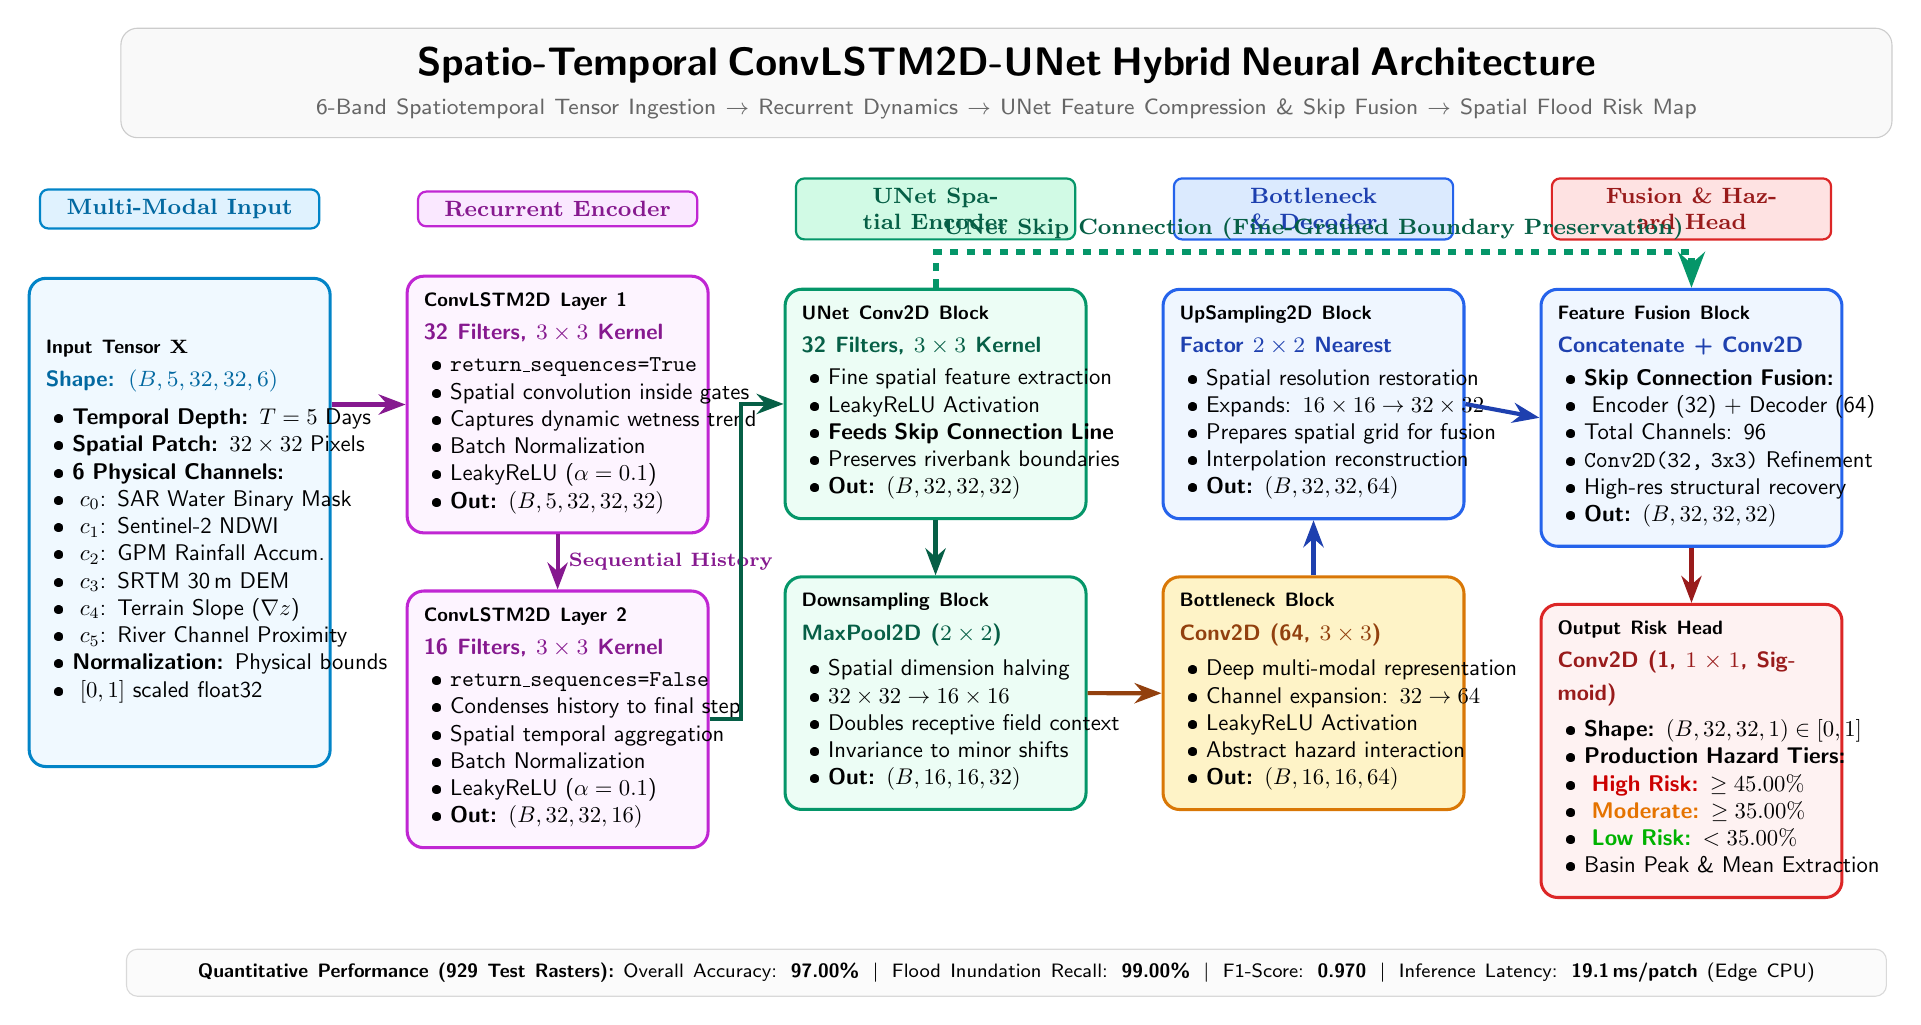
\begin{tikzpicture}[
    font=\sffamily,
    >=Stealth,
    node distance=0.6cm and 0.9cm,
    card/.style={
        rectangle, rounded corners=6pt, line width=1.1pt,
        inner sep=6pt, text width=3.4cm, align=left
    },
    banner/.style={
        rectangle, rounded corners=3pt, line width=0.8pt,
        inner sep=3.5pt, text width=3.3cm, align=center, font=\bfseries\footnotesize
    },
    flow/.style={
        ->, line width=1.5pt
    }
]

% ==================== TITLE BANNER ====================
\node[draw=gray!40, fill=gray!5, rounded corners=6pt, inner sep=7pt, text width=22cm, align=center] (title) at (10.5, 6.8) {
    {\Large\bfseries Spatio-Temporal ConvLSTM2D-UNet Hybrid Neural Architecture}\\[2pt]
    {\footnotesize\color{gray!80!black}6-Band Spatiotemporal Tensor Ingestion $\to$ Recurrent Dynamics $\to$ UNet Feature Compression \& Skip Fusion $\to$ Spatial Flood Risk Map}
};

% ==================== COLUMN 1: INPUT TENSOR ====================
\node[banner, draw=inputborder, fill=inputhead, text=inputtext] (in_head) at (0, 5.2) {
    Multi-Modal Input
};

\node[card, draw=inputborder, fill=inputbg, below=of in_head, minimum height=6.2cm] (in_card) {
    {\bfseries\scriptsize Input Tensor $\mathbf{X}$}\\
    {\footnotesize\color{inputtext}\textbf{Shape: $(B, 5, 32, 32, 6)$}}\\[4pt]
    \scalebox{0.82}{
        \begin{tabular}{@{\textbullet~}l}
        \textbf{Temporal Depth:} $T=5$ Days\\
        \textbf{Spatial Patch:} $32 \times 32$ Pixels\\
        \textbf{6 Physical Channels:}\\
        ~$c_0$: SAR Water Binary Mask\\
        ~$c_1$: Sentinel-2 NDWI\\
        ~$c_2$: GPM Rainfall Accum.\\
        ~$c_3$: SRTM 30\,m DEM\\
        ~$c_4$: Terrain Slope ($\nabla z$)\\
        ~$c_5$: River Channel Proximity\\
        \textbf{Normalization:} Physical bounds\\
        ~$[0, 1]$ scaled float32
        \end{tabular}
    }
};

% ==================== COLUMN 2: CONVLSTM2D ENCODER ====================
\node[banner, draw=lstmborder, fill=lstmhead, text=lstmtext] (lstm1_head) at (4.8, 5.2) {
    Recurrent Encoder
};

\node[card, draw=lstmborder, fill=lstmbg, below=of lstm1_head] (lstm1_card) {
    {\bfseries\scriptsize ConvLSTM2D Layer 1}\\
    {\footnotesize\color{lstmtext}\textbf{32 Filters, $3 \times 3$ Kernel}}\\[3pt]
    \scalebox{0.82}{
        \begin{tabular}{@{\textbullet~}l}
        \texttt{return\_sequences=True}\\
        Spatial convolution inside gates\\
        Captures dynamic wetness trend\\
        Batch Normalization\\
        LeakyReLU ($\alpha=0.1$)\\
        \textbf{Out:} $(B, 5, 32, 32, 32)$
        \end{tabular}
    }
};

\node[card, draw=lstmborder, fill=lstmbg, below=0.7cm of lstm1_card] (lstm2_card) {
    {\bfseries\scriptsize ConvLSTM2D Layer 2}\\
    {\footnotesize\color{lstmtext}\textbf{16 Filters, $3 \times 3$ Kernel}}\\[3pt]
    \scalebox{0.82}{
        \begin{tabular}{@{\textbullet~}l}
        \texttt{return\_sequences=False}\\
        Condenses history to final step\\
        Spatial temporal aggregation\\
        Batch Normalization\\
        LeakyReLU ($\alpha=0.1$)\\
        \textbf{Out:} $(B, 32, 32, 16)$
        \end{tabular}
    }
};

% ==================== COLUMN 3: UNET ENCODER & DOWNSAMPLING ====================
\node[banner, draw=unetborder, fill=unethead, text=unettext] (unet_enc_head) at (9.6, 5.2) {
    UNet Spatial Encoder
};

\node[card, draw=unetborder, fill=unetbg, below=of unet_enc_head] (unet_enc_card) {
    {\bfseries\scriptsize UNet Conv2D Block}\\
    {\footnotesize\color{unettext}\textbf{32 Filters, $3 \times 3$ Kernel}}\\[3pt]
    \scalebox{0.82}{
        \begin{tabular}{@{\textbullet~}l}
        Fine spatial feature extraction\\
        LeakyReLU Activation\\
        \textbf{Feeds Skip Connection Line}\\
        Preserves riverbank boundaries\\
        \textbf{Out:} $(B, 32, 32, 32)$
        \end{tabular}
    }
};

\node[card, draw=unetborder, fill=unetbg, below=0.7cm of unet_enc_card] (down_card) {
    {\bfseries\scriptsize Downsampling Block}\\
    {\footnotesize\color{unettext}\textbf{MaxPool2D ($2 \times 2$)}}\\[3pt]
    \scalebox{0.82}{
        \begin{tabular}{@{\textbullet~}l}
        Spatial dimension halving\\
        $32 \times 32 \to 16 \times 16$\\
        Doubles receptive field context\\
        Invariance to minor shifts\\
        \textbf{Out:} $(B, 16, 16, 32)$
        \end{tabular}
    }
};

% ==================== COLUMN 4: BOTTLENECK & DECODER ====================
\node[banner, draw=decodeborder, fill=decodehead, text=decodetext] (dec_head) at (14.4, 5.2) {
    Bottleneck \& Decoder
};

\node[card, draw=decodeborder, fill=decodebg, below=of dec_head] (dec_card) {
    {\bfseries\scriptsize UpSampling2D Block}\\
    {\footnotesize\color{decodetext}\textbf{Factor $2 \times 2$ Nearest}}\\[3pt]
    \scalebox{0.82}{
        \begin{tabular}{@{\textbullet~}l}
        Spatial resolution restoration\\
        Expands: $16 \times 16 \to 32 \times 32$\\
        Prepares spatial grid for fusion\\
        Interpolation reconstruction\\
        \textbf{Out:} $(B, 32, 32, 64)$
        \end{tabular}
    }
};

\node[card, draw=bottleborder, fill=bottlebg, below=0.7cm of dec_card] (bottle_card) {
    {\bfseries\scriptsize Bottleneck Block}\\
    {\footnotesize\color{bottletext}\textbf{Conv2D (64, $3 \times 3$)}}\\[3pt]
    \scalebox{0.82}{
        \begin{tabular}{@{\textbullet~}l}
        Deep multi-modal representation\\
        Channel expansion: $32 \to 64$\\
        LeakyReLU Activation\\
        Abstract hazard interaction\\
        \textbf{Out:} $(B, 16, 16, 64)$
        \end{tabular}
    }
};

% ==================== COLUMN 5: FEATURE FUSION & OUTPUT ====================
\node[banner, draw=outborder, fill=outhead, text=outtext] (out_head) at (19.2, 5.2) {
    Fusion \& Hazard Head
};

\node[card, draw=decodeborder, fill=decodebg, below=of out_head] (fusion_card) {
    {\bfseries\scriptsize Feature Fusion Block}\\
    {\footnotesize\color{decodetext}\textbf{Concatenate + Conv2D}}\\[3pt]
    \scalebox{0.82}{
        \begin{tabular}{@{\textbullet~}l}
        \textbf{Skip Connection Fusion:}\\
        ~Encoder (32) + Decoder (64)\\
        Total Channels: 96\\
        \texttt{Conv2D(32, 3x3)} Refinement\\
        High-res structural recovery\\
        \textbf{Out:} $(B, 32, 32, 32)$
        \end{tabular}
    }
};

\node[card, draw=outborder, fill=outbg, below=0.7cm of fusion_card] (out_card) {
    {\bfseries\scriptsize Output Risk Head}\\
    {\footnotesize\color{outtext}\textbf{Conv2D (1, $1 \times 1$, Sigmoid)}}\\[3pt]
    \scalebox{0.82}{
        \begin{tabular}{@{\textbullet~}l}
        \textbf{Shape:} $(B, 32, 32, 1) \in [0, 1]$\\
        \textbf{Production Hazard Tiers:}\\
        ~\textcolor{red!80!black}{\textbf{High Risk:}} $\ge 45.00\%$\\
        ~\textcolor{orange!90!black}{\textbf{Moderate:}} $\ge 35.00\%$\\
        ~\textcolor{green!70!black}{\textbf{Low Risk:}} $< 35.00\%$\\
        Basin Peak \& Mean Extraction
        \end{tabular}
    }
};

% ==================== FLOW ARROWS ====================
% Input -> ConvLSTM1
\draw[flow, draw=lstmtext] (in_card.east |- lstm1_card.west) -- (lstm1_card.west);

% ConvLSTM1 -> ConvLSTM2
\draw[flow, draw=lstmtext] (lstm1_card.south) -- (lstm2_card.north)
    node[midway, right, font=\scriptsize\bfseries, color=lstmtext] {Sequential History};

% ConvLSTM2 -> UNet Encoder
\draw[flow, draw=unettext] (lstm2_card.east) -- ++(0.4, 0) |- (unet_enc_card.west);

% UNet Encoder -> Downsampling
\draw[flow, draw=unettext] (unet_enc_card.south) -- (down_card.north);

% Downsampling -> Bottleneck
\draw[flow, draw=bottletext] (down_card.east) -- (bottle_card.west);

% Bottleneck -> Decoder
\draw[flow, draw=decodetext] (bottle_card.north) -- (dec_card.south);

% Decoder -> Fusion
\draw[flow, draw=decodetext] (dec_card.east) -- (fusion_card.west);

% Fusion -> Output Head
\draw[flow, draw=outtext] (fusion_card.south) -- (out_card.north);

% ==================== SKIP CONNECTION (ARC OVER TOP) ====================
\draw[->, line width=2.2pt, draw=unetborder, dashed]
    (unet_enc_card.north) -- ++(0, 0.45) -| (fusion_card.north)
    node[pos=0.25, above, font=\footnotesize\bfseries, color=unettext] {UNet Skip Connection (Fine-Grained Boundary Preservation)};

% ==================== FOOTNOTE / METRICS BANNER ====================
\node[draw=gray!30, fill=gray!3, rounded corners=4pt, inner sep=5pt, text width=22cm, align=center] at (10.5, -4.5) {
    {\scriptsize\bfseries Quantitative Performance (929 Test Rasters):}~{\scriptsize Overall Accuracy: \textbf{97.00\%} $\,\vert\,$ Flood Inundation Recall: \textbf{99.00\%} $\,\vert\,$ F1-Score: \textbf{0.970} $\,\vert\,$ Inference Latency: \textbf{19.1\,ms/patch} (Edge CPU)}
};

\end{tikzpicture}
\end{document}
